\documentclass[ignorenonframetext,]{beamer}
\usetheme{CambridgeUS}
\setbeamertemplate{caption}[numbered]
\setbeamertemplate{caption label separator}{:}
\setbeamercolor{caption name}{fg=normal text.fg}
\usepackage{amssymb,amsmath}
\usepackage{ifxetex,ifluatex}
\usepackage{fixltx2e} % provides \textsubscript
\usepackage{lmodern}
\ifxetex
  \usepackage{fontspec,xltxtra,xunicode}
  \defaultfontfeatures{Mapping=tex-text,Scale=MatchLowercase}
  \newcommand{\euro}{€}
\else
  \ifluatex
    \usepackage{fontspec}
    \defaultfontfeatures{Mapping=tex-text,Scale=MatchLowercase}
    \newcommand{\euro}{€}
  \else
    \usepackage[T1]{fontenc}
    \usepackage[utf8]{inputenc}
      \fi
\fi
% use upquote if available, for straight quotes in verbatim environments
\IfFileExists{upquote.sty}{\usepackage{upquote}}{}
% use microtype if available
\IfFileExists{microtype.sty}{\usepackage{microtype}}{}
\usepackage{longtable,booktabs}
\usepackage{caption}
% These lines are needed to make table captions work with longtable:
\makeatletter
\def\fnum@table{\tablename~\thetable}
\makeatother
\usepackage{graphicx}
\makeatletter
\def\maxwidth{\ifdim\Gin@nat@width>\linewidth\linewidth\else\Gin@nat@width\fi}
\def\maxheight{\ifdim\Gin@nat@height>\textheight0.8\textheight\else\Gin@nat@height\fi}
\makeatother
% Scale images if necessary, so that they will not overflow the page
% margins by default, and it is still possible to overwrite the defaults
% using explicit options in \includegraphics[width, height, ...]{}
\setkeys{Gin}{width=\maxwidth,height=\maxheight,keepaspectratio}

% Comment these out if you don't want a slide with just the
% part/section/subsection/subsubsection title:
\AtBeginPart{
  \let\insertpartnumber\relax
  \let\partname\relax
  \frame{\partpage}
}
\AtBeginSection{
  \let\insertsectionnumber\relax
  \let\sectionname\relax
  \frame{\sectionpage}
}
\AtBeginSubsection{
  \let\insertsubsectionnumber\relax
  \let\subsectionname\relax
  \frame{\subsectionpage}
}

\setlength{\parindent}{0pt}
\setlength{\parskip}{6pt plus 2pt minus 1pt}
\setlength{\emergencystretch}{3em}  % prevent overfull lines
\setcounter{secnumdepth}{0}
\usepackage[russian]{babel}
\usepackage{dcolumn}
\usepackage{diagrams}
\DeclareMathOperator{\plim}{plim}
\newcommand{\e}{\varepsilon}

\title{Эконометрика. Лекция 9. Эндогенность}
\date{}

\begin{document}
\frame{\titlepage}

\begin{frame}{Разложение в сумму не однозначно}

\[
4 = 3 + 1
\]

\[
4 = 2 + 2
\]

\end{frame}

\begin{frame}{Несколько верных форм одной модели}

Модель А: \[
y_i=2x_i + \varepsilon_i
\]

Модель Б: \[
y_i=3x_i + u_i
\]

Модели А и Б эквивалентны, если \(\varepsilon_i=x_i+u_i\)

\end{frame}

\begin{frame}{Свойства МНК. Если\ldots{}}

Если:

модель представлена в форме

\[
y_i=\beta_1 + \beta_2 x_i + \beta_3 z_i + \varepsilon_i
\] где \(E(\varepsilon_i | X)=0\) и {[}другие предпосылки{]}

\end{frame}

\begin{frame}{Свойства МНК. То\ldots{}}

То:

Оценки МНК состоятельны \[
\hat{\beta} \to \beta
\]

и несмещены \[
E(\hat{\beta})=\beta
\]

\end{frame}

\begin{frame}{Смысл предпосылки \(E(\varepsilon_i | X)=0\)}

Среднее значение \(\varepsilon_i\) не зависит от значений объясняющих
переменных и равно нулю.

В частности, \[
E(\varepsilon_i | X)=0   \; \Rightarrow 
\begin{cases}
E(\varepsilon_i)=0 \\ 
Cov(x_i,\varepsilon_i)=0
\end{cases}
\]

\end{frame}

\begin{frame}{Последствия нарушения предпосылки}

Если \(Cov(x_i, \varepsilon_i) \neq 0\), то оценки МНК несостоятельны:

\[
\hat{\beta} \not \to \beta
\]

и смещены \[
E(\hat{\beta}) \neq \beta
\]

\end{frame}

\begin{frame}{Пример у неоновой доски}

\[
y_i=2+3x_i + \varepsilon_i
\] где \(Var(x_i)=4\), \(Var( \varepsilon_i)=3\),
\(Cov(x_i , \varepsilon_i) = -2\)

Найдите \(\plim \hat{\beta}_2\)

\end{frame}

\begin{frame}{Полезные обозначения}

Выборочная ковариация \[
sCov(x,y)=\frac{\sum (x_i-\bar{x})(y_i-\bar{y})}{n-1}
\]

Выборочная дисперсия \[
sVar(x)=\frac{\sum (x_i-\bar{x})^2}{n-1}
\]

\end{frame}

\begin{frame}{Полезный факт}

Следствие закона больших чисел

Если выборка \((x_i,y_i)\) случайна, то

\[
\plim sCov(x,y) = Cov(x_i,y_i)
\]

\[
\plim sVar(x) = Var(x_i)
\]

\end{frame}

\begin{frame}{Эндогенность}

Ситуация \(Cov(x_i, \varepsilon_i) \neq 0\) называется эндогенностью

\end{frame}

\begin{frame}{Зачем возиться с эндогенностью?}

У любой модели есть форма записи, в которой \(E(\varepsilon_i|X)=0\).

Зачем нужны те формы записи, в которых \(E(\varepsilon_i|X) \neq 0\)?

\end{frame}

\begin{frame}{Два ответа}

\begin{itemize}
\item
  Если модель используется для прогнозирования, то формы записи с
  эндогенностью не нужны.
\item
  В некоторых случаях форма записи с эндогенностью легче
  интерпретируется.
\end{itemize}

\end{frame}

\begin{frame}{Причины эндогенности в перекрёстных выборках}

\begin{itemize}
\item
  Ошибка измерения регрессора
\item
  Пропущенный регрессор
\end{itemize}

\end{frame}

\begin{frame}{Ошибка измерения регрессора. Исходная форма модели.}

Модель в форме А: \[
y_i=\beta_1 + \beta_2 x_i + \varepsilon_i
\] и \(Cov(x_i, \varepsilon_i)=0\).

Наблюдаем \(y_i\) и \(x_i^*=x_i + u_i\), где \(u_i\), ошибка измерения
регрессора \(x_i\), не зависит от \(x_i\) и \(\varepsilon_i\)

\end{frame}

\begin{frame}{Ошибка измерения регрессора. Вывод другой формы модели.}

Подставим \(x_i=x_i^*-u_i\) в форму А и получим:

\[
y_i=\beta_1 + \beta_2 (x_i^*-u_i) + \varepsilon_i
\]

и модель в форме Б: \[
y_i=\beta_1 + \beta_2 x_i^*  + w_i, \; w_i=\varepsilon_i - \beta_2 u_i
\]

\end{frame}

\begin{frame}{Эндогенность в форме Б:}

\[
y_i=\beta_1 + \beta_2 x_i^*  + w_i, \; w_i=\varepsilon_i - \beta_2 u_i
\]

В форме Б: \[
Cov(x_i^*,w_i)=Cov(x_i+u_i,\varepsilon_i - \beta_2 u_i)=-\beta_2 Var(u_i) \neq 0
\]

МНК оценки для формы Б несостоятельны

\end{frame}

\begin{frame}{Пример у неоновой доски}

\[
y_i= 2 + 3x_i + \varepsilon_i
\]

Регрессор \(x_i\) ненаблюдаем

Наблюдаем \(x_i^*=x_i+u_i\), \(Var(x_i)=9\), \(Var(u_i=4)\),
\(Var(\varepsilon_i)=1\).

К чему стремится МНК оценка модели
\(\hat{y}_i = \hat{\beta}_1 + \hat{\beta}_2 x_i^*\)?

\end{frame}

\begin{frame}{Мораль:}

Модель с ошибкой измерения регрессора:

\[
y_i= \beta_1 + \beta_2 x_i + \varepsilon_i, \; \text{ где наблюдаем } x_i^*=x_i+u_i
\]

\begin{itemize}
\itemsep1pt\parskip0pt\parsep0pt
\item
  Хотим оценить \(\beta_2\), т.е. на сколько растёт \(y_i\) при росте
  настоящего \(x_i\) на единицу
\end{itemize}

\end{frame}

\begin{frame}{Мораль. МНК для нашей цели не состоятелен.}

При МНК оценивании регрессии \[
\hat{y}_i = \hat{\beta}_1 + \hat{\beta}_2 x_i^*
\] получаем оценку \(\hat{\beta}_2\) несостоятельную для \(\beta_2\)

\begin{itemize}
\itemsep1pt\parskip0pt\parsep0pt
\item
  МНК оценивает на сколько растёт \(y_i\) при росте померянного
  \(x_i^*\) (включающего ошибку) на единицу
\end{itemize}

\end{frame}

\begin{frame}{Пропущенная объясняющая переменная}

Хотим оценить форму записи А: \[
y_i=\beta_1 + \beta_2 x_i + \beta_3 d_i + \e_i
\] где \(Cov(x_i,d_i)\neq 0\), \(Cov(x_i,\e_i)=0\), \(Cov(d_i,\e_i)=0\).

Не наблюдаем \(d_i\).

\end{frame}

\begin{frame}{Пропущенная объясняющая переменная.}

Форма записи Б: \[
y_i=\beta_1 + \beta_2 x_i + u_i\, \; u_i=\beta_3 d_i + \e_i
\]

Эндогенность: \[
Cov(x_i,u_i)=Cov(x_i,\beta_3 d_i + \e_i)=\beta_3 Cov(x_i, d_i)
\]

\end{frame}

\begin{frame}{Пример у неоновой доски}

\[
y_i= 2 + 3x_i -2d_i + \varepsilon_i
\]

Регрессор \(d_i\) ненаблюдаем.

\(Var(x_i)=Var(d_i)=9\), \(Var(\varepsilon_i)=1\), \(Cov(x_i,d_i)=-6\).

К чему стремится МНК оценка модели
\(\hat{y}_i = \hat{\beta}_1 + \hat{\beta}_2 x_i\)?

\end{frame}

\begin{frame}{Мораль}

Модель пропущенным регрессором:

\[
y_i= \beta_1 + \beta_2 x_i + \beta_3 d_i + \varepsilon_i, \; \text{ регрессор } d_i \text{ не наблюдаем}
\]

\begin{itemize}
\itemsep1pt\parskip0pt\parsep0pt
\item
  Хотим оценить \(\beta_2\), т.е. на сколько растёт \(y_i\) при росте
  \(x_i\) на единицу и фиксированном \(d_i\)
\end{itemize}

\end{frame}

\begin{frame}{Мораль. МНК для нашей цели не состоятелен.}

При МНК оценивании регрессии \[
\hat{y}_i = \hat{\beta}_1 + \hat{\beta}_2 x_i
\] получаем оценку \(\hat{\beta}_2\) несостоятельную для \(\beta_2\)

\begin{itemize}
\itemsep1pt\parskip0pt\parsep0pt
\item
  МНК оценивает на сколько растёт \(y_i\) при росте \(x_i\) на единицу
  (и сопряженных с этим изменениях в \(d_i\))
\end{itemize}

\end{frame}

\begin{frame}{Инструментальные переменные}

Хотим состоятельно оценить \(\beta_2\) в форме записи:

\[
y_i=\beta_1 + \beta_2 x_i + \e_i, \; Cov(x_i,\e_i)\neq 0
\]

Возможный выход: найти ``инструментальные переменные'' \(z_i\):

\begin{itemize}
\item
  \(Cov(z_i, \e_i)=0\)
\item
  \(Cov(z_i, x_i) \neq 0\)
\end{itemize}

\end{frame}

\begin{frame}{Как использовать инструментальные переменные?}

Модель: \[
y_i = \beta_1 + \beta_2 x_i + \beta_3 d_i + \e_i
\] где \(Cov(x_i,\e_i) \neq 0\) и \(Cov(d_i,\e_i)=0\).

\end{frame}

\begin{frame}{Двухшаговый МНК:}

Шаг 1. Построить регрессию каждого \(x_i\) коррелированного с \(\e_i\)
на инструментальные переменные. Получить \(\hat{x}_i\).

Шаг 2. Оценить исходную модель заменив \(x_i\) на \(\hat{x}_i\)

\[
y_i = \beta_1 + \beta_2 \hat{x}_i + \beta_3 d_i + u_i
\]

Получаем \(\hat{\beta}_1^{IV}\), \(\hat{\beta}_2^{IV}\) и
\(\hat{\beta}_3^{IV}\)

\end{frame}

\begin{frame}{Метод инструментальных переменных}

Метод двухшагового МНК также называют методом инструментальных
переменных:

\[
\hat{\beta}^{2OLS}=\hat{\beta}^{IV}
\]

\end{frame}

\begin{frame}{Простейший случай двухшагового МНК}

\[
y_i=\beta_1+\beta_2 x_i + \e_i
\]

МНК: \[
\hat{\beta}_2^{OLS}=\frac{sCov(x,y)}{sVar(x)}
\] Метод инструментальных переменных: \[
\hat{\beta}_2^{IV}=\frac{sCov(z,y)}{sCov(z,x)}
\]

\end{frame}

\begin{frame}{Пример у неоновой доски. Спасение.}

\[
y_i= \beta_1 + \beta_2 x_i + \beta_3 d_i + \varepsilon_i
\]

Регрессор \(d_i\) ненаблюдаем.

\(Var(x_i)=Var(d_i)=9\), \(Var(\varepsilon_i)=1\), \(Cov(x_i,d_i)=-6\).

К чему стремится IV оценка модели
\(\hat{y}_i = \hat{\beta}_1 + \hat{\beta}_2 x_i\)?

Есть инструментальная переменная \(z_i\), \(Cov(x_i,z_i)=1\).

\end{frame}

\begin{frame}{Как найти инструментальную переменую?}

Инструментальная переменная \(z_i\) для регрессора \(x_i\) может влиять
на \(y_i\) через через регрессор \(x_i\), но не через ошибку \(\e_i\).

\end{frame}

\begin{frame}{Связи инструментальной переменной}

Модель с эндогенностью: \[
y_i = \beta_1 + \beta_2 x_i + \e_i
\]

\[
\begin{diagram}
x_i  & \rTo  & y_i \\
\uTo & \ruTo &     \\
\e_i &       &     \\
\end{diagram}
\]

монтажерам: а потом превратить в \[
\begin{diagram}
z_i &\rTo & x_i  & \rTo  & y_i \\
    &     & \uTo & \ruTo &     \\
    &     & \e_i &       &    \\
\end{diagram}
\]

\end{frame}

\begin{frame}{Статистическая связь не означает причинно-следственной}

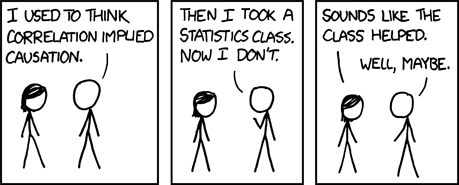
\includegraphics{correlation.png}

\end{frame}

\begin{frame}{Типы данных}

\begin{itemize}
\item
  Данные наблюдений
\item
  Данные экспериментов
\end{itemize}

\end{frame}

\begin{frame}{Данные наблюдений}

Каждое утро выхожу на балкон и записываю, вижу ли я людей с зонтами и
идет ли дождь

\begin{longtable}[c]{@{}rrr@{}}
\toprule
Утро & Люди с зонтами & Дождь\tabularnewline
\midrule
\endhead
1 & 0 & 1\tabularnewline
2 & 1 & 1\tabularnewline
3 & 0 & 0\tabularnewline
4 & 1 & 1\tabularnewline
\bottomrule
\end{longtable}

\end{frame}

\begin{frame}{Данные экспериментов}

Каждое утро подбрасываю монетку и в зависимости от монетки, либо беру
зонт, либо не беру

\begin{longtable}[c]{@{}rrrr@{}}
\toprule
Утро & Монетка & Я с зонтом & Дождь\tabularnewline
\midrule
\endhead
1 & Орёл & 0 & 1\tabularnewline
2 & Решка & 1 & 1\tabularnewline
3 & Решка & 1 & 0\tabularnewline
4 & Орёл & 0 & 1\tabularnewline
\bottomrule
\end{longtable}

\end{frame}

\begin{frame}{Эксперименты}

\begin{itemize}
\item
  Искусственные
\item
  Естественные
\end{itemize}

\end{frame}

\begin{frame}{Стратегия идентификации причинно-следственных связей}

\begin{itemize}
\item
  Придумать идеальный эксперимент
\item
  Найти похожий естественный эксперимент
\end{itemize}

\end{frame}

\begin{frame}{Данные наблюдений --- примеры}

\begin{itemize}
\item
  Публикационное смещение
\item
  Выборочное исправление ошибок
\item
  Байка про Абрахама Вальда
\end{itemize}

\end{frame}

\begin{frame}{Публикационное смещение}

\begin{itemize}
\itemsep1pt\parskip0pt\parsep0pt
\item
  У сенсационного результата больше шансов быть опубликованным
\end{itemize}

\end{frame}

\begin{frame}{Выборочное исправление ошибок}

Исследователь Вениамин верит в \(H_0\), но проводит честное исследование

\begin{itemize}
\itemsep1pt\parskip0pt\parsep0pt
\item
  нет ошибок
\item
  есть ошибка, смещающая результат в пользу \(H_0\) Вениамин обрадуется
  результату и, вероятно, не заметит ошибку
\item
  есть ошибка, смещающая результат в пользу \(H_a\) Вениамин будет
  удивлен, трижды перепроверит работу и найдёт ошибку
\end{itemize}

\end{frame}

\begin{frame}{История про Абрахама Вальда}

здесь схематичная картинка днища самолёта с дырочками от пуль

где-то плотность дырочек должна быть выше, где-то ниже

\end{frame}

\end{document}
